\documentclass[10pt,letterpaper]{article}
\usepackage[utf8]{inputenc}
\usepackage{amsmath}
\usepackage{amsfonts}
\usepackage{amssymb}
\usepackage{graphicx}
\usepackage{tabularx}
\usepackage[left=2cm,right=2cm,top=2cm,bottom=2cm]{geometry}
\author{Trent Baker, Logan Bonney, Cody Stoner, Madison Fichtner}
\title{ESOF 322 - Programming Assignment 2}

\newcommand{\usecasetwocol}[1]{
\begin{center}
	\begin{tabularx}{0.8\textwidth}{| X X |}
		\hline
		#1 \\
		\hline
	\end{tabularx}
\end{center}
}

\newcommand{\usecasedescription}[1]{
\begin{center}
	\begin{tabularx}{0.8\textwidth}{l X}
		#1
	\end{tabularx}
\end{center}
}

\newcommand{\usecase}[2]{
\usecasedescription{#1}
\usecasetwocol{#2}
}

\begin{document}
\maketitle

\usecase{Use Case: & The Play \\
	Actors: & Current Player \\
	Goals: & For player to roll both dice to receive n from the sum of the dice, move icon n spaces on the board, according to space, player may buy property, pay rent, or pay taxes. If  doubles are rolled, they move n spaces, then repeat. If doubles are thrown 3 times in a  turn, player icon goes to jail. \\
	Steps: &  }{
	The player rolls dice & \\
	&The system returns the dice as an length 2 array \\
	The player moves that many spaces forward on the board &\\
	&If the player passed the GO space, they are credited \$200.00 \\
	&The system takes actions based on the space the player landed on \\
	If the dice roll was doubles, add one to that players double counter, and take another turn&}

\usecase{Use Case: & Buying Property \\
	Actors: & Current Player \\
	Goals: & When player lands on property, they may purchase said property. Player receives the title deed. If player does not want property, property is put up for auction in which they can also bid, highest bidder wins property. \\
	Preconditions: & Property must not already be owned by another player. \\
	Steps: & }{The player lands on an unclaimed space &\\
	The player chooses to buy the property at its current price or not &\\
	&If not, pass the deed to auction \\
	&If the player chooses to buy the property, the player is debited the current price, and  given the property}

\usecase{Use Case: & Property Auction \\
	Actors: & All players \\
	Goals: & All players must be able to bid on property that was passed on by the current player whos turn it is. \\
	Preconditions: & Property must have no been bought by player who landed on property \\
	Steps: &  }{Any player places a bid &\\
	&If that bid was higher than the previous bid, that player is placed in the lead \\
	If 30 seconds pass without a bid, the player in the lead is debited the current bid and given the deed&}

\usecase{Use Case: & Selling Property \\
	Actors: & Current Player, Player Who’s Buying \\
	Goals: & Allow the current player to sell one of their already owned properties to another player. If property being sold is mortgaged, the purchasing player must either lift the mortgage at	once by paying the mortgage plus 10\% interest; or pay for the property as well as pay the bank 10\% interest at the time of purchase, and then pay to lift the mortgage plus  10\% interest at a later time. \\
	Preconditions: & Current player must own said property. \\
	Steps: &  }{The player chooses a property of theirs to sell &\\
	&If the property is mortgaged the player is given the option to pay it off and then sell it \\
	The seller chooses a price to sell it for& \\
	&Each player is given the option to buy it \\
	If a player chooses to buy it, the properties’ ownership is transferred to the new owner and they pay the price to the seller&}

\usecase{Use Case: & Paying Rent \\
	Actors: & Current Player, Property Owning Player \\
	Goals: & When current player lands on property owned by another player, the property owner receives x amount of \$ from current player specified on title deed for how developed the  property may be. If property is mortgaged, no rent can be collected. Rent doubles if property owner owns all of that group of properties, and is increased based on how improved property is. \\
	Preconditions: & Property landed on must be already owned by a player \\
	Steps: &  }{The player lands on the property of another player & \\
	&The server checks if the property is mortgaged \\
	If it is not then the rent is calculated and the player that landed on pays it to the owner of the property&}

\usecase{Use Case: & Income Tax \\
	Actors: & Current Player \\
	Goals: & If current player lands on income tax spot, they must either pay \$200 or pay 10\% of net worth (cash on hand, printed prices of mortgaged and unmortgaged property, and cost  price of all buildings owned) \\
	Steps: &  }{The player lands on income tax &\\
	The player may choose to pay \$200 or 10\% if their net worth &\\
	&If the player chooses 10\% then the server sums their net worth and the player pays 10\% of it}

\usecase{Use Case: & Jail \\
	Actors: & Current Player \\
	Goals: & Current player goes to jail under 2 conditions: land on space “Go to Jail” or throws doubles three times. Player can get out of jail if: they throw doubles on any of next three  turns, paying \$50 before rolling dice on any of 3 turns. Must pay \$50 if it is third turn in  jail. On turn that player gets out of jail (by rolling doubles, or paying) player moves  forward the number rolled on the doubles, or rolls dice after paying. Player may buy and  sell property, sell houses and hotels, and receive rent while in jail. \\
	Steps: &  }{The player lands on the “Go to Jail” space or throws a third double in a row& \\
	&The player is moved to jail and their turn is ended \\
	The player may pay \$50 dollars or attempt to roll doubles to get out of jail. If it is their third turn in jail they are fined \$50 dollars &\\
	&If the player payed or was fined \$50 they roll and move. If they rolled doubles they move by the number rolled.}

\usecase{Use Case: & Free Parking \\
	Actors: & Current Player \\
	Goals: & If player lands on “Free Parking” spot, they receive no money, property, or reward of any kind (they do nothing). \\
	Steps: &  }{&}

\usecase{Use Case: & Buying Houses \\
	Actors: & Current Player \\
	Goals: & Player may build houses on any property of color group, but must build on unimproved  properties of this or any other fully owned color group (must build evenly on properties). Price of house is shown on deed of property. May build up to four houses on each property. \\
	Preconditions: & Player must own all property in group \\
	Steps: &  }{The user attempts to build a house &\\
	&The server checks if all properties of the color are owned \\
	&If they are, the system checks if the other properties in the color group have greater than or equal to number of houses \\
	If they do, the system debits the house cost from the player, The system places a house&}

\usecase{Use Case: & Buying Hotels \\
	Actors: & Current Player \\
	Goals: & Player may buy a hotel (price specified on title deed) that replaces houses on property. Only one hotel may be on each property. \\
	Preconditions: & Player must have four houses on specified property  \\
	Steps: &  }{Player begins buying a hotel on a street &\\
	&The system checks if there are four houses on the street \\
	&If there are, the system checks if the number of hotels is maxed,  \\
	If it isn’t, The system debits the hotel cost from the user, removes the houses, and places a hotel&}

\usecase{Use Case: & Mortgages \\
	Actors: & Current Player \\
	Goals: &  No rent can be collected on mortgaged properties or utilities, but rent can be collected on unmortgaged properties in the same group. In order to lift the mortgage, the owner must pay the Bank the amount of the mortgage plus 10\% interest. When all the properties of a color-group are no longer mortgaged, the owner may begin to buy back houses at full price.  \\
	Preconditions: & Player must own said property \\
	Steps: & }{The user begins mortgaging an unimproved deed &\\
	&The system changes the deeds mortgage status to true and gives the player the deeds mortgage price}

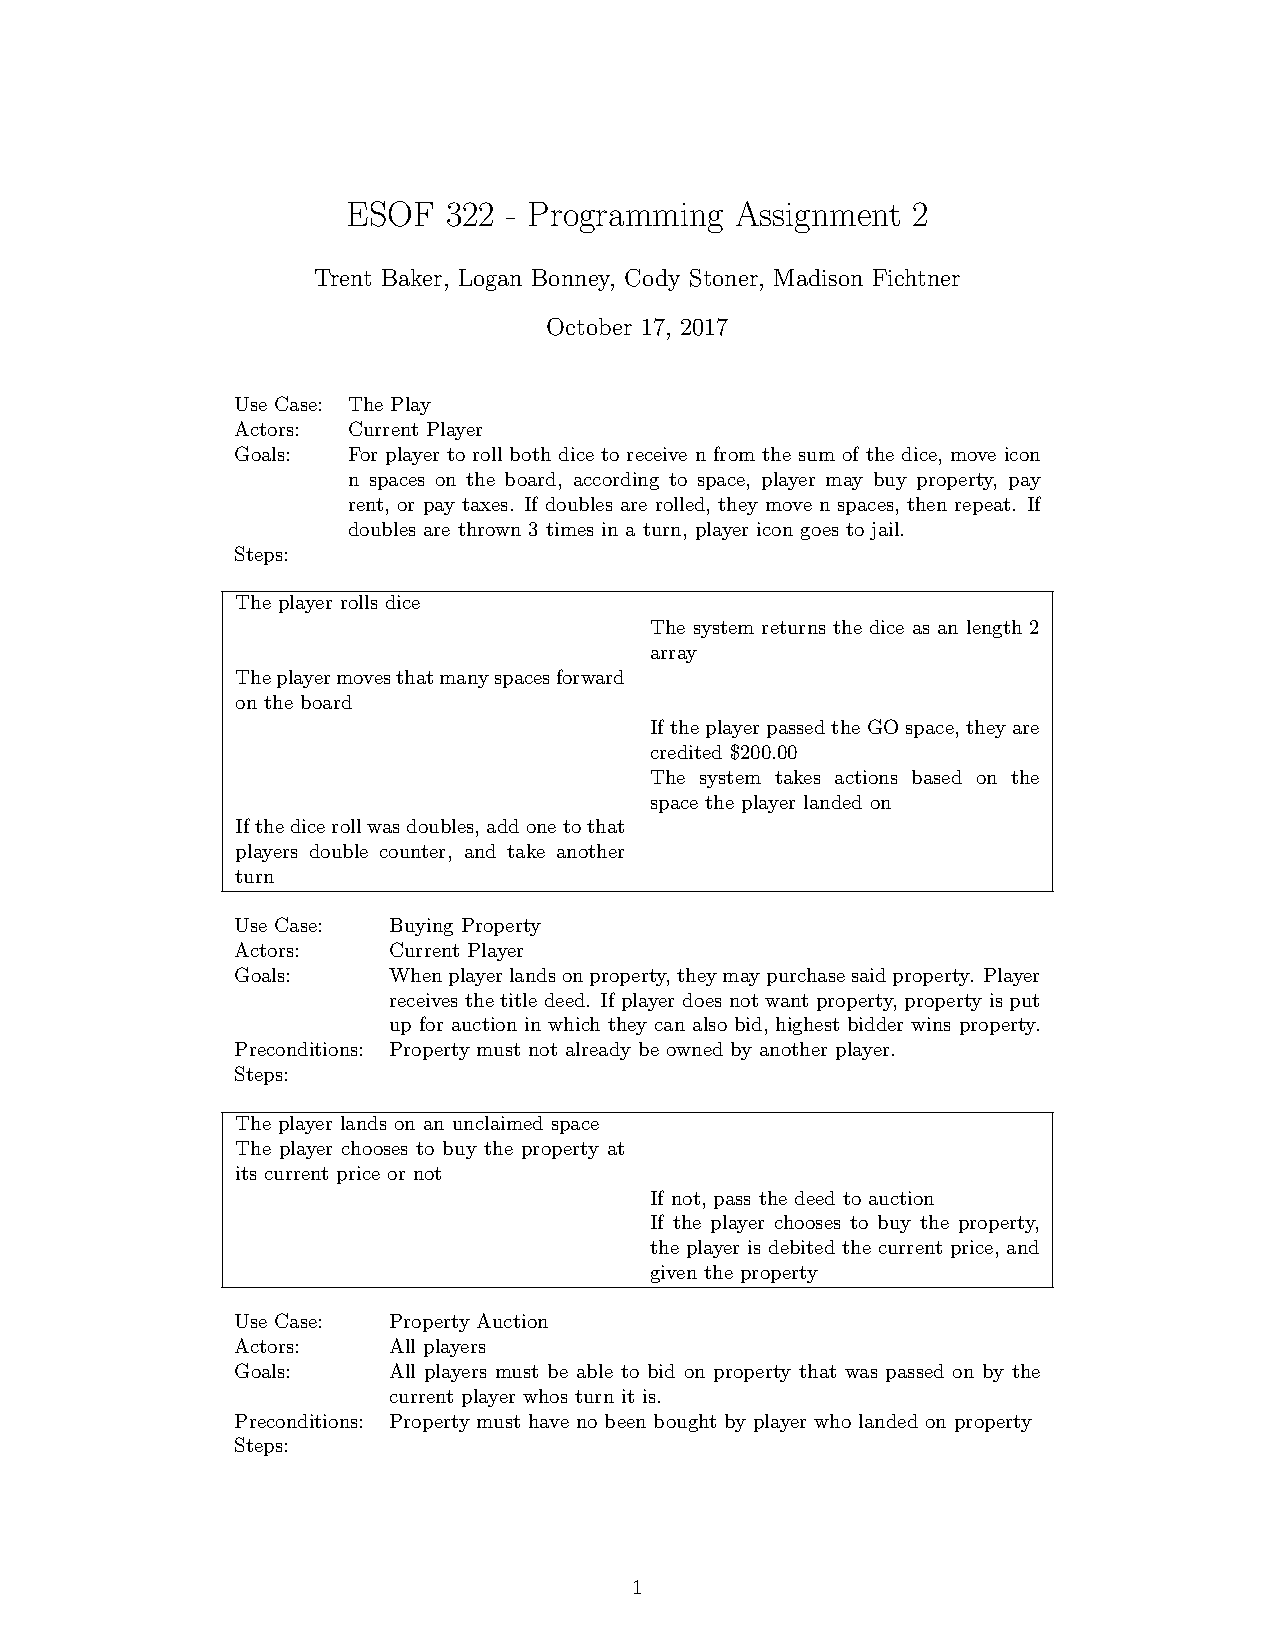
\includegraphics[width=\textwidth]{ESOF322_PA2}
\end{document}
